\section{Lecture 15}

\subsection{Quantum Error-Correction: Intro}
A long time ago, in the 1950s, there were analog computers. Rather than storing data as
0s and 1s, you store it as real numbers (these can be mechanical systems or electrical systems).
A noiseless analog computer is very powerful; adding up arbitrary precision real numbers is very powerful.
However, in the real world, these are noisy, which actually makes them computationally equivalent to digital computers. 
And later we realized that digital computers are far more scalable than analog ones, so that's why our computer systems are digital today!

Back when quantum computing was just starting up, people would scared it would be analog computing all over again.
Peter Shor invented the Shor code to fix this problem.

\subsection{Classical Error-Correction}
We have a bitstring with characters in $\{0, 1\}$ sitting in our hard drive. Suppose that cosmic ray comes in
and spontaneously flips some bits. To protect against this, the simplest thing to do is the \textbf{repetition code}, e.g.
storing the logical bit $0$ as $000$ and the logical bit $1$ as $111$. This redundancy allows us to protect
against some errors. Suppose you see $101$; we would use \emph{majority rule} and declare the bit was $1$, encoding as $111$.
The probability that it was initially $000$ is small (specifically $\frac{1}{8}$).

What's the probability that we get this wrong? If the probability of any individual bit getting flipped is $p \ll 1$ (independently),
the probability of any bit wrong is $O(p^2)$, which is very small.

\subsection{Shor Code}
The quantum error-correction problem seems impossible because there are infinitely many errors; we will later show that 
it actually is possible using the \textbf{Shor Code}.

For now, let us assume that
the only possible error that could occur on a qubit is an $X$ gate (the quantum bit-flip). For a single bit state
we'd like to encode a logical qubit as
$\ket{\tilde{\psi}} \mapsto \ket{\psi}\ket{\psi}\ket{\psi}$,
but this is impossible due to no-cloning.
We have to settle for the CNOT copying we saw prior:
\[ \ket{\tilde{0}} \mapsto \ket{000}, \ket{\tilde{1}} \mapsto \ket{111} \]
And we can encode a general state with linearity
\[ \ket{\tilde{\psi}} = \alpha \ket{\tilde{0}} + \beta \ket{\tilde{1}} \mapsto \alpha \ket{000} + \beta \ket{111} \]
We say that we want to correct at most one bitflip $X$ (the other qubits have the identity applied to them).

After noise, we want to correct the error using the same ``majority rule algorithm.'' If we had a nonsuperpositional computational state,
then we could measure in computational basis and be done. The problem is we cannot measure without destroying information.
So instead, we build the following circuit, calling our noisy codeword $\ket{x} = \ket{x_1, x_2, x_3}$.
\begin{center}
\begin{quantikz}
   \lstick[wires=3]{$\ket{x}$} & \ctrl{3} & \qw & \qw & \qw & \qw\\ 
                      & \qw & \ctrl{2} & \ctrl{3} & \qw & \qw \\ 
                      & \qw & \qw  & \qw & \ctrl{2} & \qw \\
   \lstick{$\ket{0}$} & \targ{} & \targ{} & \qw & \qw & \qw & \meter{} \\ 
   \lstick{$\ket{0}$} & \qw & \qw & \targ{} & \targ{} & \qw & \meter{} \\ 
\end{quantikz}
\end{center}
This maps a computational basis state
\[ \ket{x_1, x_2, x_3} \ket{00} \mapsto \ket{x_1, x_2, x_3} \ket{x_1 \oplus x_2, x_2 \oplus x_3} \]
and then measures the ancilla bits. Let us analyze the cases for the resulting state:

\noindent
\textbf{Case 1.} If there was no error, we have $\ket{00}$ on the ancilla bits and measure $00$.
The state collapses back to $\alpha \ket{000} + \beta \ket{111}$.

\noindent
\textbf{Case 2.} If there was a $X_1$ error, we have $\ket{10}$ on the ancilla bits and measure $10$.
The state collapses to $\alpha \ket{100} + \beta \ket{011}$.

\noindent
\textbf{Case 3.} If there was a $X_2$ error, we have $\ket{11}$ on the ancilla bits and measure $11$.
The state collapses to $\alpha \ket{010} + \beta \ket{101}$.

\noindent
\textbf{Case 4.} If there was an $X_3$ error, we have $\ket{01}$ on the ancilla bits and measure $01$.
The state collapses to $\alpha \ket{001} + \beta \ket{110}$.

In all cases, it's clear what's left to do, just apply $X_i$ to the bit $i$ if it was flipped, otherwise don't do anything.
The measurement on the ancilla bits is called a \textbf{Syndrome Measurement}.
Recall the phase flip operator
\[ Z = \begin{pmatrix}
    1 & 0 \\ 0 & -1
\end{pmatrix} = 1 \ketbra{0} - 1 \ketbra{1} \]
Applying the syndrome measurement e.g. measuring $s$ on the first ancilla qubit
is the same as measuring $(-1)^s$ in the basis $Z_1 Z_2$. To see this, note that measuring with
$Z_1$ on state $\ket{x_1, x_2, x_3}$ will yield $(-1)^{x_1}$. Thus, multiplying the two will XOR the bits, yielding $Z_1Z_2 = (-1)^{x_1 \oplus x_2}$.
We can then summarize:
\begin{center}
\begin{tabular}{ | c | c | c | c | }
    Error & Ancilla measurement & Syndrome measurement & Error correction \\ \hline
    $I$ & 00 & $Z_1 Z_2 = 1, Z_2 Z_3 = 1$ & $I$ \\ 
    $X_1$ & 10 & $Z_1 Z_2 = -1, Z_2 Z_3 = 1$ & $X_1$ \\
    $X_2$ & 11 & $Z_1 Z_2 = -1, Z_2 Z_3 = -1$ & $X_2$ \\
    $X_3$ & 01 & $Z_1 Z_2 = 1, Z_2 Z_3 = -1$ & $X_3$ \\
\end{tabular}
\end{center}

But $X$ gates are not the only things that could happen to qubits. What if a $Z$ gate was sneakily applied instead?
\[ Z_1 (\alpha \ket{000} + \beta \ket{111}) = \alpha \ket{000} - \beta \ket{111} = \tilde{Z}\qty(\alpha \ket{\tilde{0}} + \beta \ket{\tilde{1}}) \]
There's no way to distinguish an error from a different logical state. We need to find a different code.
But there is symmetry between $X$ and $Z$: they are the same under a change of basis. So, we
can then define the repetition code as:
\[ \ket{\tilde{+}} \mapsto \ket{+++}, \quad \ket{\tilde{-}} \mapsto \ket{---} \]
Because we have this duality between them, we get the same table
\begin{center}
    \begin{tabular}{ | c | c | c | c | }
        Error & Ancilla measurement & Syndrome measurement & Error correction \\ \hline
        $I$ & $++$ & $X_1 X_2 = 1, X_2 X_3 = 1$ & $I$ \\ 
        $X_1$ & $-+$ & $X_1 X_2 = -1, X_2 X_3 = 1$ & $Z_1$ \\
        $X_2$ & $--$ & $X_1 X_2 = -1, X_2 X_3 = -1$ & $Z_2$ \\
        $X_3$ & $+-$ & $X_1 X_2 = 1, X_2 X_3 = -1$ & $Z_3$ \\
\end{tabular}
\end{center}
But now by the same logic, we cannot correct bit flip errors.
To fix this, we can now perform code concatenation, i.e. encode our logical bits with the phase flip code
and then the bit flip code. This yields a 9-qubit code:
\begin{align*}
    \ket{\tilde{\tilde{+}}} &\mapsto \ket{\tilde{+}} \ket{\tilde{+}} \ket{\tilde{+}} \mapsto \frac{1}{2\sqrt{2}}\qty(\ket{000} + \ket{111})^{\otimes 3} \\
    \ket{\tilde{\tilde{-}}} &\mapsto \ket{\tilde{-}} \ket{\tilde{-}} \ket{\tilde{-}} \mapsto \frac{1}{2\sqrt{2}}\qty(\ket{000} - \ket{111})^{\otimes 3}
\end{align*}
On decoding, we first error-correct within each bit-flip code (i.e. $\ket{x_1,x_2,x_3}, \ket{x_4,x_5,x_6}, \ket{x_7,x_8,x_9}$):
\[ Z_1 Z_2, Z_2 Z_3, Z_4 Z_5, Z_5 Z_6, Z_7 Z_8, Z_8 Z_9 \]
nd apply $X$ gates as necessary. What about phase-flip errors? Notice that
\[ Z_1 \ket{\tilde{\tilde{\psi}}} = Z_2 \ket{\tilde{\tilde{\psi}}} = Z_3 \ket{\tilde{\tilde{\psi}}} = \tilde{Z}_{\tilde{1}} \ket{\tilde{\tilde{\psi}}} \]
This is similar for $Z_{4,5,6}$ and $Z_{7,8,9}$ with $\tilde{Z}_{\tilde{2}}$ and $\tilde{Z}_{\tilde{3}}$.
This means that to correct for phase flip errors in the first bit-flip code, we just have to measure $\tilde{X}_{\tilde{1}}\tilde{X}_{\tilde{2}}$. What do these operators actually mean as physical operators? Well, they flip the entire logical bit:
\begin{align*}
    \tilde{X}_{\tilde{1}} \ket{\tilde{0} \tilde{0} \tilde{0}} &= \ket{\tilde{1} \tilde{0} \tilde{0}} \\
    \tilde{X}_{\tilde{1}} \ket{000000000} &= \ket{111000000}
\end{align*}
Thus, we have $\tilde{X}_{\tilde{1}} = X_1 X_2 X_3$, $\tilde{X}_{\tilde{2}} = X_4 X_5 X_6$, and $\tilde{X}_{\tilde{3}} = X_7 X_8 X_9$.
So on the outer code, we are measuring
\begin{align*}
    \tilde{X}_{\tilde{1}}\tilde{X}_{\tilde{2}} &= X_1 X_2 X_3 X_4 X_5 X_6 \\
    \tilde{X}_{\tilde{2}}\tilde{X}_{\tilde{3}} &= X_4 X_5 X_6 X_7 X_8 X_9
\end{align*}
Hence, the summary table for phase-flip error correction is 
\begin{center}
    \begin{tabular}{ | c | c | c | c | }
        Error & Syndrome measurement & Error correction \\ \hline
        $I$ & $X_1 X_2 X_3 X_4 X_5 X_6 = 1, \quad X_4 X_5 X_6 X_7 X_8 X_9 = 1$ & $I$ \\ 
        $Z_1Z_2Z_3$ & $X_1 X_2 X_3 X_4 X_5 X_6 = -1, \quad X_4 X_5 X_6 X_7 X_8 X_9 = 1$ & $Z_1$ \\
        $Z_4Z_5Z_6$ & $X_1 X_2 X_3 X_4 X_5 X_6 = -1, \quad X_4 X_5 X_6 X_7 X_8 X_9 = -1$ & $Z_4$ \\
        $Z_7Z_8Z_9$ & $X_1 X_2 X_3 X_4 X_5 X_6 = 1, \quad X_4 X_5 X_6 X_7 X_8 X_9 = -1$ & $Z_7$ \\
\end{tabular}
\end{center}
Thus, we have an quantum error correcting code that
can correct any 1-qubit bit or phase flip. This is known as the $9$-qubit \textbf{Shor code}, depicted by the circuit below:
\begin{center}
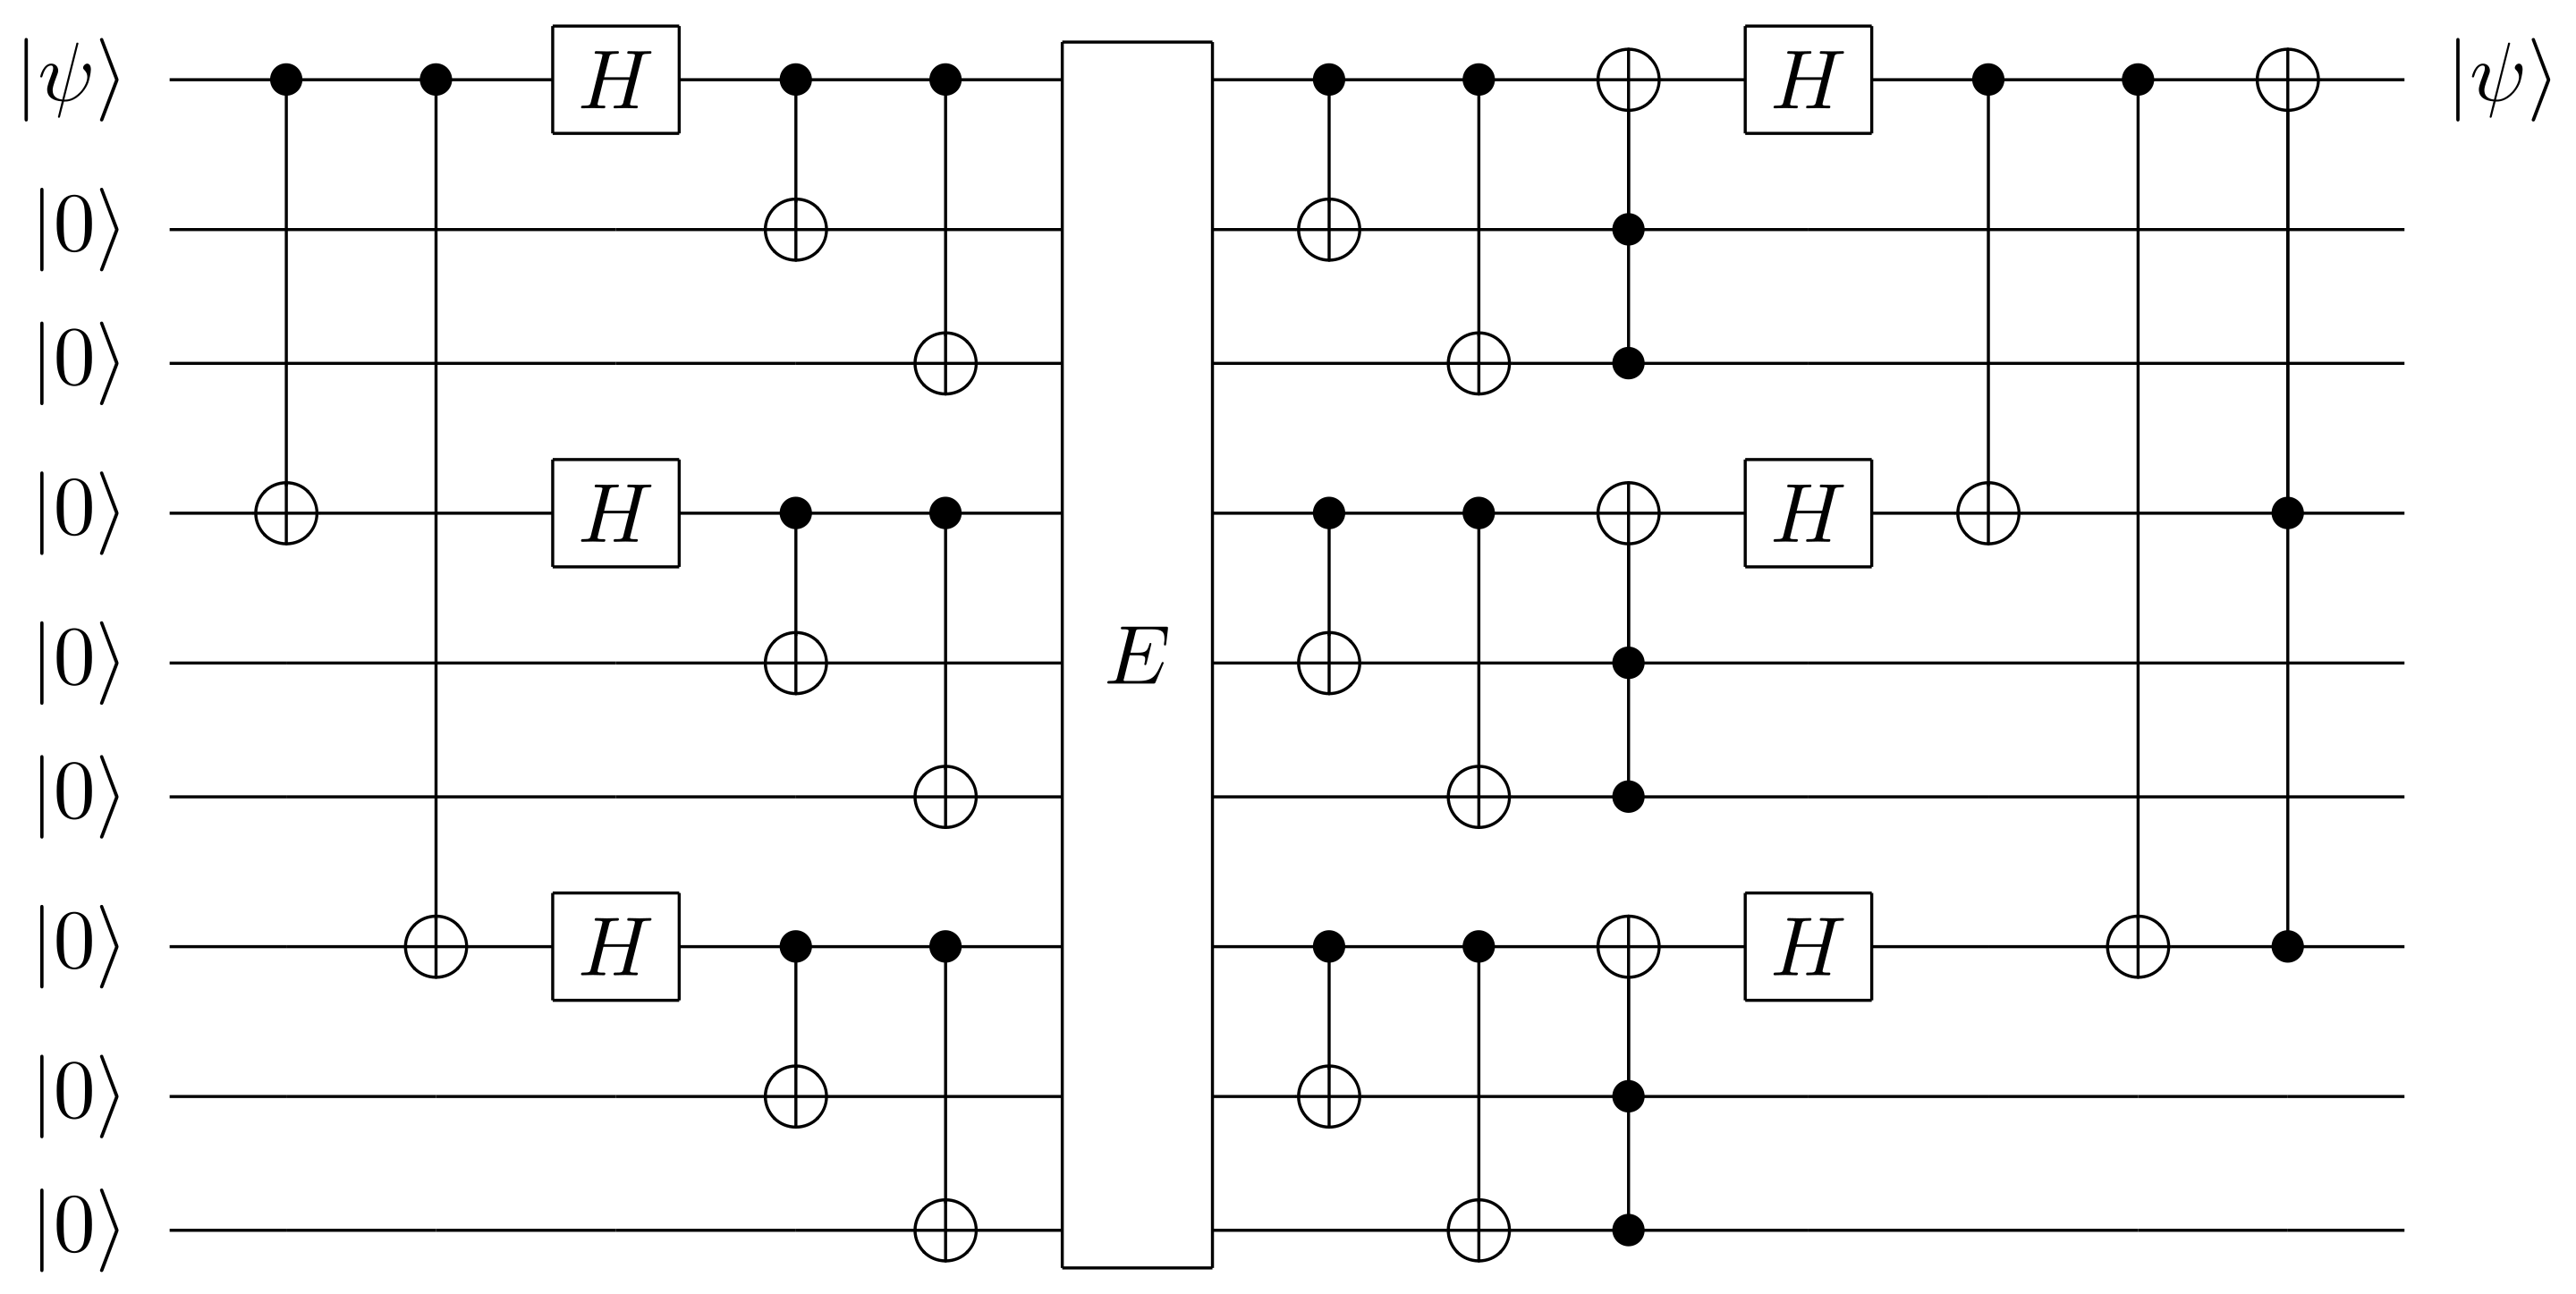
\includegraphics[width=\textwidth*2/3]{../images/lec15_shor.png} 
\end{center}
where $E$ is where any bit or phase flip error may occur. Using the Shor code, we can in fact correct
all the pauli errors, e.g. consider $Y = i XZ$, and the $i$ is irrelevant (we will drop the global phase for simplicity) so \[ Y \ket{\tilde{\tilde{\psi}}} = X_k \tilde{Z}_k \ket{\tilde{\tilde{\psi}}} \mapsto \tilde{Z}_k \ket{\tilde{\tilde{\psi}}} \mapsto \ket{\tilde{\tilde{\psi}}}\]
This is due to how we can correct errors one at a time.

\subsection{General Quantum Errors}
It turns out the Shor code can error-correct any general error introduced by a quantum channel.
Recall the Kraus operator representation
\begin{align*}
    \mathcal{N}(\rho) &= \sum_i K_i \rho K_i^{\dagger}
\end{align*}
We will consider only a single state, because if we can correct a single state, we can correct an ensemble.
\[ \mathcal{N}\qty(\ketbra{\tilde{\tilde{\psi}}}) = \sum_i K_i \ketbra{\tilde{\tilde{\psi}}} K_i^{\dagger} \]
We will take $K_j$ acting on only one qubit $j$; but since it is a 2x2 matrix, it can be written
as a linear combination of the Pauli basis:
\[ K_j \ket{\tilde{\tilde{\psi_j}}} = \alpha I \ket{\tilde{\tilde{\psi_j}}} + \beta X_j \ket{\tilde{\tilde{\psi_j}}} + \gamma Y_j \ket{\tilde{\tilde{\psi_j}}} + \delta Z_j \ket{\tilde{\tilde{\psi_j}}} \]
So, any error can be thought of as a superposition of Pauli errors.
But syndrome measurement gives a different outcome for all the errors $I, X_i, Y_i, Z_i$.
Doing this measurement destroys the superposition and reduces it to one of the Pauli matrices. But, we know how to deal with an error pattern of one of any of these.
So the Shor code works in general.
